\clearpage
\section{Method references, implementation map, and sanity checks}
\label{sec:method-audit}
The main text presents the methods used to generate the relative-entropy
data and the reasons for choosing them. Here we collect the independent
constructions and numerical evidence supporting that choice.
This appendix separates the published ingredients from their assembly
in this project. Equation numbers in the reading guide refer to the
linked arXiv versions. The companion \texttt{METHOD\_REFERENCES.md}
gives the same reading route, source paths, and executable commands.
The full reproducibility archive contains the Python implementation;
the Overleaf archive contains the report and validation records.

\subsection{Definitions of the state-quality diagnostics}
\label{sec:validation-metrics}
To judge the quality of a normalized candidate $\ket{\psi}$, we compute
its mean energy $E_\psi=\bra{\psi}H\ket{\psi}$ and eigenstate residual
\begin{equation}
 \eta_\psi=\|(H-E_\psi)\ket{\psi}\|_2
 =\sqrt{\bra{\psi}H^2\ket{\psi}-E_\psi^2}.
 \label{eq:eigenresidual}
\end{equation}
The residual vanishes for an exact eigenstate. We also check symmetry and energy
ordering, because a small residual alone does not identify the desired
primary. The vector norm is $\|v\|_2=(\sum_i|v_i|^2)^{1/2}$.

\subsection{Compact-boson wavefunction and Haldane--Shastry checks}
\label{sec:boson-sanity}
We evaluate Eq.~\eqref{eq:bosonpolynomial} independently of the
logarithmic correlator implementation and compare normalized vectors.
For each fixed $N$, charge pair $(a,b)$, and endpoint $W$, let $\psi$
be the normalized vector obtained by directly evaluating the
Laughlin/Jastrow polynomial in Eq.~\eqref{eq:bosonpolynomial}
(\texttt{polynomial\_state} in the code). Let $\phi$ be the normalized
conformal-block vector obtained by exponentiating the logarithmic
amplitudes in Eq.~\eqref{eq:logblock} (\texttt{vertex\_state}). Both
vectors represent the same chosen primary, with identical coordinates,
endpoint and occupation basis. Define their phase-aligned amplitude error
\begin{equation}
 e_{\rm amp}(\psi,\phi)=
 \max_O\left|\psi(O)e^{-i\arg\langle\phi|\psi\rangle}-\phi(O)\right|.
 \label{eq:amplitudeerror}
\end{equation}
The argument $\arg$ is the phase of the complex overlap. This comparison
checks that two implementations produce the same wavefunction, including
its phases and normalization. To test an independent spectral property
of that wavefunction, we also examine its eigenstate residual.

\paragraph{Why use the Haldane--Shastry Hamiltonian?}
The choice is specific to the exponent-two Jastrow states on the uniform
circle used here. Their half-filled vacuum is exactly the ground state
of the Haldane--Shastry (HS) spin chain, whose continuum description is
the compact boson at the $SU(2)_1$ radius. The conformal-block vacuum
and its relation to HS are given in Ref.~\cite{Herwerth}, Sec.~II A,
Eq.~(10), and Sec.~III A, Eq.~(37). This makes HS a natural additional
benchmark for our three explicit lattice states. In our energy convention,
the Hamiltonian is
\begin{equation}
 H_{\rm HS}=\left(\frac{\pi}{N}\right)^2
 \sum_{j<k}\frac{\bm S_j\cdot\bm S_k}{\sin^2[\pi(j-k)/N]},
 \qquad \bm S_j=(X_j,Y_j,Z_j)/2.
 \label{eq:HHS}
\end{equation}
Here $X,Y,Z$ are Pauli matrices, so each site is a spin one-half.
For each normalized state we compute
\begin{equation}
 E_{\rm HS}=\langle\psi|H_{\rm HS}|\psi\rangle,\qquad
 \eta_{\rm HS}=\|(H_{\rm HS}-E_{\rm HS})\ket{\psi}\|_2.
\end{equation}
This is Eq.~\eqref{eq:eigenresidual} with the Hamiltonian specified.
A small $\eta_{\rm HS}$ tests stationarity under HS; it does not by
itself identify the CFT primary or establish its conformal weights.
For the three states at $N=8,10,12$, the largest residual at strict
infinity is $6.21\times10^{-15}$. The excited-state residuals at
$W=10^8$ range from $4.60\times10^{-9}$ to $6.30\times10^{-9}$,
showing the small departure from an HS eigenstate introduced by retaining
the original finite endpoint.

All three boson vectors are constructed directly from the conformal-block
or polynomial amplitudes before applying this test. The HS Hamiltonian
is used only as a diagnostic: it neither generates these vectors nor
enters the relative entropy, which is calculated from their reduced
density matrices. Its use here is not a requirement of the continuum
relative-entropy theory and does not extend automatically to other
compactification radii or lattice geometries.

\begin{table}[htbp]\centering\small
\begin{tabular}{rlrrrr}\toprule
$N$ & State & $e_{\rm amp}(\infty)$ & $e_{\rm amp}(10^8)$ & $\eta(\infty)$ & $\eta(10^8)$\\\midrule
8 & $00$ & $9.30\times10^{-16}$ & $9.30\times10^{-16}$ & $1.04\times10^{-15}$ & $1.04\times10^{-15}$ \\
8 & $ss$ & $1.04\times10^{-15}$ & $8.50\times10^{-16}$ & $1.43\times10^{-15}$ & $5.97\times10^{-9}$ \\
8 & $3s,s$ & $4.38\times10^{-16}$ & $5.00\times10^{-16}$ & $8.02\times10^{-16}$ & $6.30\times10^{-9}$ \\
10 & $00$ & $2.86\times10^{-15}$ & $2.86\times10^{-15}$ & $1.58\times10^{-15}$ & $1.58\times10^{-15}$ \\
10 & $ss$ & $1.18\times10^{-15}$ & $1.14\times10^{-15}$ & $1.32\times10^{-15}$ & $5.22\times10^{-9}$ \\
10 & $3s,s$ & $1.46\times10^{-15}$ & $2.01\times10^{-15}$ & $9.82\times10^{-16}$ & $5.35\times10^{-9}$ \\
12 & $00$ & $2.89\times10^{-15}$ & $2.89\times10^{-15}$ & $6.21\times10^{-15}$ & $6.21\times10^{-15}$ \\
12 & $ss$ & $1.70\times10^{-15}$ & $2.24\times10^{-15}$ & $5.58\times10^{-15}$ & $4.60\times10^{-9}$ \\
12 & $3s,s$ & $1.88\times10^{-15}$ & $1.83\times10^{-15}$ & $5.11\times10^{-15}$ & $4.66\times10^{-9}$ \\
\bottomrule\end{tabular}

\caption{Direct polynomial versus logarithmic conformal-block evaluation
for the three canonical boson states. Here $\psi$ is the normalized
direct Laughlin/Jastrow polynomial vector of Eq.~\eqref{eq:bosonpolynomial},
and $\phi$ is the normalized conformal-block vector obtained by
exponentiating Eq.~\eqref{eq:logblock}. Each comparison uses the same
$N$, primary and endpoint $W$ for both vectors. The two amplitude-error
columns give $e_{\rm amp}(\psi,\phi)$ from Eq.~\eqref{eq:amplitudeerror};
the two residual columns apply Eqs.~\eqref{eq:eigenresidual} and
\eqref{eq:HHS} to $\psi$.
All vectors are normalized, $z_j=e^{2\pi i j/N}$, and the endpoint is
either strict infinity or $10^8$. The finite-endpoint residuals quantify
the perturbation retained to match the original Laughlin implementation.
No interval length or mixing probability enters these whole-state tests.}
\label{tab:bosoncanonical}
\end{table}

\clearpage
\subsection{Independent Ising constructions used for validation}
\label{sec:ising-independent}
The production reduced states use the exact fermion covariance method
of Sec.~\ref{sec:ising-production}. The full-vector constructions below
provide independent checks of that input: conformal blocks for $I,\eps$,
and conformal-block-seeded Lanczos projection for $\sigma$.

The chiral Ising fields are $1,\chi,\sigma$ with weights $0,1/2,1/16$;
$\chi$ is a Majorana fermion. Their fusion rules are
\begin{equation}
 \sigma\times\sigma=1+\chi,\qquad
 \chi\times\chi=1,\qquad \chi\times\sigma=\sigma.
\end{equation}

\subsubsection{Vacuum block: fusion data become spin amplitudes}
For the vacuum, the auxiliary correlator is
$\langle0|\sigma(z_1)\cdots\sigma(z_{2N})|0\rangle_{\bm p}$.
The subscript $\bm p$ chooses its intermediate fusion channels.
\begin{enumerate}
\item Use $2N$ spin fields on the circle,
$z_r=\exp[i\theta_r]$ with $\theta_r=\pi r/N$, $r=1,\ldots,2N$.
Pair $(z_{2j-1},z_{2j})$. Each pair fuses to identity ($m_j=0$) or
fermion ($m_j=1$), defining a physical spin with $Z_j=(-1)^{m_j}$.
\item Label the successive intermediate channels by bits
$\bm p=(p_1,\ldots,p_{N-1})$, setting $p_0=p_N=0$.
The physical bits are $m_j=p_{j-1}\mathbin{\mathrm{xor}}p_j$.
Thus $\sum_jm_j$ is even. The construction spans the even sector of the
physical spin parity $P=\prod_j Z_j$.
\item Enumerate binary strings $\bm q=(q_1,\ldots,q_{N-1})$ and define
$s_1=1$, $s_j=\prod_{k<j}(1-2q_k)$.
Split the field coordinates into two groups
$l_{\bm q}(j)=2j-(1+s_j)/2$ and
$l'_{\bm q}(j)=2j-(1-s_j)/2$. Each group contains one field from each pair.
Calculate the positive weight
\begin{equation}
 A_{\bm q}=\prod_{j>k}
 \left[\sin\frac{\theta_{l_{\bm q}(j)}-\theta_{l_{\bm q}(k)}}2
 \sin\frac{\theta_{l'_{\bm q}(j)}-\theta_{l'_{\bm q}(k)}}2\right]^{1/2}.
\end{equation}
\item Define $B_{\bm p}=\sum_{\bm q}(-1)^{\bm p\cdot\bm q}A_{\bm q}$,
where the dot product is a sum of products of bits. The vacuum amplitudes
are $\psi_I(\bm m(\bm p))\propto\sqrt{B_{\bm p}}$.
The binary sign sum is a Walsh--Hadamard transform, evaluated with
$O(N2^{N-1})$ butterfly operations instead of evaluating every
$(\bm p,\bm q)$ pair separately.
The weights themselves cost $O(N^2 2^{N-1})$ operations.
\item Normalize by
$\mathcal N_I=(\sum_{\bm p}B_{\bm p})^{1/2}$, so that
$\psi_I(\bm m(\bm p))=\sqrt{B_{\bm p}}/\mathcal N_I$.
Set all odd-parity amplitudes to zero. The output is a normalized
$2^N$-component vector.
\end{enumerate}
The homogeneous choice sets the pair-displacement parameter $\delta=0$ in
\texttt{fusion\_blocks}. Ref.~\cite{Montes2017} proves that this block
vacuum is the finite-chain critical ground state. We additionally check
its energy, symmetry sector, and residual numerically.

\subsubsection{Energy primary: insert two Majorana endpoint fields}
\begin{enumerate}
\item Keep the same $2N$ spin fields, coordinates, and physical basis.
Replace the auxiliary vacuum states by Majorana states:
\begin{equation}
 \Psi_\eps(\bm p)\propto
 \langle\chi|\sigma(z_1)\cdots\sigma(z_{2N})|\chi\rangle_{\bm p}.
\end{equation}
Since the chiral Majorana has weight $1/2$, the insertion at infinity
means $\chi(\infty)=\lim_{W\to\infty}W\chi(W)$.
The two endpoints preserve even physical parity.
\item Reuse $A_{\bm q}$ and $B_{\bm p}$ from the vacuum construction.
The endpoint correlator introduces the real factor
$C_{\bm q}=\cos[(\pi/2N)\sum_j s_j]$. Compute a second sign transform
$U_{\bm p}=\sum_{\bm q}(-1)^{\bm p\cdot\bm q}A_{\bm q}C_{\bm q}$.
The explicit result is
\begin{equation}
 \psi_\eps(\bm m(\bm p))\propto
 \frac{\displaystyle\sum_{\bm q}(-1)^{\bm p\cdot\bm q}A_{\bm q}
 \cos\left(\frac\pi{2N}\sum_{j=1}^Ns_j\right)}{\sqrt{B_{\bm p}}}.
\label{eq:epsblock}
\end{equation}
\item Normalize by
$\mathcal N_\eps=(\sum_{\bm p}|U_{\bm p}|^2/B_{\bm p})^{1/2}$
and embed $\psi_\eps(\bm m(\bm p))=U_{\bm p}/(\sqrt{B_{\bm p}}\mathcal N_\eps)$
in the same spin basis.
\item Check its orthogonality to $I$, its even parity, zero momentum,
energy, and eigenstate residual. The identification with the nonchiral
primary $\eps$ uses these spectral and symmetry properties; the
auxiliary chiral endpoint fields alone do not establish that identification.
\end{enumerate}
Equation~\eqref{eq:epsblock} is the published expression in
Ref.~\cite{Montes2017}, Eqs.~(73)--(75), specialized to the uniform
circle. Its equality with the desired excited eigenstate is numerically
verified here through $N=24$; we do not replace that numerical evidence
by an unprovided general proof for arbitrary insertions.

\subsubsection{Spin primary: conformal-block-seeded Lanczos}
\label{sec:sigmamethod}
An even-parity block cannot represent the odd-parity $\sigma$ state.
Ref.~\cite{Montes2017}, Sec.~X, reports that the naive endpoint-spin and
single-fermion candidates do not directly yield the desired homogeneous
odd-sector ground state. To check the production covariance state
independently at small sizes, we construct a full-vector representative
of $\sigma$ by a Hamiltonian projection initialized from the block vacuum.
This seed and projection are our combination of the published block
vacuum and a standard eigensolver, not a formula claimed in that paper.
Here ``block-seeded'' means seeded by a conformal block; the solver is
single-vector Lanczos, not a multi-vector block-Lanczos algorithm.
The steps below specify the numerical construction, including the part
performed by the Lanczos solver~\cite{ARPACK,ScipyEigsh}.

\begin{enumerate}
\item \textbf{Prepare a seed with the required symmetry.}
Starting from normalized $\ket{I_{\rm CB}}$, set
\begin{equation}
 \ket{v_\sigma}=\sum_{j=0}^{N-1}X_j\ket{I_{\rm CB}},\qquad
 \ket{q_1}=\frac{\ket{v_\sigma}}{\|v_\sigma\|_2}.
 \label{eq:sigmaseed}
\end{equation}
Since $PX_j=-X_jP$, the seed is odd. The sum is invariant under
translation, so the seed has zero momentum. It generally contains
higher-energy odd states as well as $\sigma$; applying the summed spin
operator is not itself the final projection.
\item \textbf{Build the odd-sector Hamiltonian action.}
Retain only bit strings $\bm m$ with $\sum_jm_j$ odd, leaving
$2^{N-1}$ basis vectors. Let $H_-$ denote $H$ restricted to this basis.
For a coefficient vector $f$, its action is
\begin{equation}
 (H_-f)_{\bm m}=
 -\left[\sum_j(-1)^{m_j}\right]f_{\bm m}
 -\sum_j f_{\bm m\oplus\bm e_j\oplus\bm e_{j+1}},
 \label{eq:oddaction}
\end{equation}
where $\bm e_j$ has one bit at site $j$, $\oplus$ is bitwise exclusive-or,
and site indices are periodic. The first term is diagonal; the second
flips neighboring bits. No full $2^{N-1}$ by $2^{N-1}$ matrix is stored.
Only parity is explicitly imposed in this basis; translation symmetry
is inherited from the seed and preserved by the Hamiltonian.
\item \textbf{Generate a Krylov space.}
After $r$ basis vectors, the search space is
\begin{equation}
 \mathcal K_r=\operatorname{span}
 \{q_1,H_-q_1,\ldots,H_-^{r-1}q_1\}.
\end{equation}
Lanczos constructs orthonormal vectors $q_j$. In exact arithmetic,
with $q_0=0$ and $b_0=0$, the recurrence is
\begin{align}
 a_j&=\langle q_j|H_-|q_j\rangle,\notag\\
 \ket{w_j}&=H_-\ket{q_j}-a_j\ket{q_j}-b_{j-1}\ket{q_{j-1}},\notag\\
 b_j&=\|w_j\|_2,\qquad \ket{q_{j+1}}=\ket{w_j}/b_j.
 \label{eq:lanczos}
\end{align}
If $b_j=0$, the generated subspace is already invariant. In floating-point
arithmetic the solver also controls loss of orthogonality. The symbols
$a_j,b_j$ here are Lanczos coefficients, unrelated to the boson endpoint
labels or the leading fitting exponent $\alpha$.
\item \textbf{Select the lowest-energy combination.}
Form $(T_r)_{ij}=\langle q_i|H_-|q_j\rangle$. This small matrix is
tridiagonal, with diagonal $a_j$ and neighboring entries $b_j$.
Let $\theta_{\min}$ and $\bm y$ be its smallest eigenvalue and normalized
eigenvector. The Rayleigh--Ritz approximation is
\begin{equation}
 \ket{\sigma_N^{(r)}}=\sum_{j=1}^r y_j\ket{q_j}.
\end{equation}
It minimizes the energy within the current search space. Increasing the
space, or restarting while retaining the useful spectral information,
refines the approximation.
\item \textbf{Converge and measure the actual residual.}
The code calls \texttt{eigsh} with \texttt{k=1}, \texttt{which="SA"},
the seed as \texttt{v0}, and \texttt{tol=2e-12}. It uses implicitly
restarted Lanczos~\cite{ScipyEigsh}. The requested solver tolerance is
not an absolute bound on $\eta$: after convergence we independently
evaluate Eq.~\eqref{eq:eigenresidual} using the original Hamiltonian.
\item \textbf{Identify and validate the primary.}
Normalize the vector, restore zero entries on even bit strings, and
check $P=-1$, zero momentum, orthogonality to $I,\eps$, and the energy
$E_\sigma=-2\cot[\pi/(2N)]$. The vanishing large-$N$ gap has scaling
dimension $1/8$, identifying the $(1/16,1/16)$ primary.
Our explicit construction checks use
$e_P=\|(P+1)\sigma_N\|_2$ and
$e_{\mathsf T}=\|(\mathsf T-1)\sigma_N\|_2$ for the two symmetry errors.
\end{enumerate}

The spectral projection underlying these steps can also be written as
\begin{equation}
 \ket{\sigma_N}=\lim_{\tau\to\infty}
 \frac{e^{-\tau(H-E_*)}\ket{q_1}}
 {\|e^{-\tau(H-E_*)}\ket{q_1}\|_2}.
 \label{eq:projection}
\end{equation}
Here $\tau$ is imaginary time and $E_*$ is an arbitrary reference energy.
The normalized seed has an expansion into odd-sector eigenstates;
provided its $\sigma$ coefficient is nonzero, higher energies are
suppressed relative to the lowest one. Lanczos implements the search
without explicitly exponentiating $H$.
The measured squared seed overlap
$F_{\rm seed}=|\langle\sigma_N|q_1\rangle|^2$ is approximately
$0.986,0.983,0.981,0.979,0.977$ at $N=6,8,10,12,16$.
At $N=16$, the recorded projected-state residual is
$2.70\times10^{-12}$.
The complete size-by-size residual and independent-state checks appear
in Appendix~\ref{sec:ising-spin-validation}; the largest recorded residual is
$1.99\times10^{-11}$ at $N=12$. Thus the solver tolerance must not be
quoted as the achieved absolute residual.

This method obtains the required lattice primary using both a conformal
block and the Hamiltonian. A pure endpoint conformal-block formula for
the periodic $\sigma$ state remains unestablished here.


\subsection{Comparisons with the original lattice implementations}
\label{sec:state-comparisons}
We define squared fidelity $F=|\langle\psi|\phi\rangle|^2$ for normalized
vectors, infidelity $1-F$, and matrix error
$\|M\|_F=(\Tr M^\dagger M)^{1/2}$. The most useful energy ratio uses
\emph{excitation gaps}, since ratios of extensive total energies are
insensitive to the excitation:
\begin{equation}
 E_I=-2\csc\frac\pi{2N},\quad E_\sigma=-2\cot\frac\pi{2N},\quad
 E_\eps=E_I+8\sin\frac\pi{2N},\quad
 R_E=\frac{E_\eps-E_I}{E_\sigma-E_I}=8\cos^2\frac\pi{4N}.
 \label{eq:gaps}
\end{equation}
The continuum limit is $R_E\to8$, from dimensions $1$ and $1/8$.
With the velocity $v=2$ of Eq.~\eqref{eq:Hising}, the relation
$E_a-E_I\sim(2\pi v/N)(h_a+\bar h_a)$ identifies
the $\eps$ and $\sigma$ dimensions as $1$ and $1/8$, respectively.

\begin{table}[htbp]\centering\small
\begin{tabular}{rrlrrrr}\toprule
$N$ & $D_{\rm bond}$ & State & Infidelity & $|E_{\rm puMPS}-E_{\rm CB}|$ & $\eta_{\rm puMPS}$ & $\|\Delta\rho_4\|_F$\\\midrule
10 & 8 & $I$ & $1.65\!\times\!10^{-9}$ & $1.95\!\times\!10^{-8}$ & $4.88\!\times\!10^{-4}$ & $1.91\!\times\!10^{-6}$ \\
10 & 8 & $\sigma$ & $3.97\!\times\!10^{-8}$ & $5.18\!\times\!10^{-7}$ & 0.0026512 & $6.23\!\times\!10^{-6}$ \\
10 & 8 & $\varepsilon$ & $1.64\!\times\!10^{-7}$ & $1.93\!\times\!10^{-6}$ & 0.0048855 & $2.46\!\times\!10^{-5}$ \\
16 & 14 & $I$ & $2.62\!\times\!10^{-10}$ & $2.81\!\times\!10^{-9}$ & $1.81\!\times\!10^{-4}$ & $2.33\!\times\!10^{-6}$ \\
16 & 14 & $\sigma$ & $6.34\!\times\!10^{-8}$ & $7.61\!\times\!10^{-7}$ & 0.0031009 & $2.89\!\times\!10^{-6}$ \\
16 & 14 & $\varepsilon$ & $3.99\!\times\!10^{-7}$ & $4.30\!\times\!10^{-6}$ & 0.007004 & $1.46\!\times\!10^{-5}$ \\
\bottomrule\end{tabular}

\caption{Fresh full-vector comparisons with archived puMPS checkpoints.
$D_{\rm bond}$ is the MPS bond dimension, distinct from relative entropy.
The seed is $1234+N$ in the archived optimization. $I$ and $\eps$ use pure
CB vectors, while $\sigma$ uses Eq.~\eqref{eq:projection}. All vectors
are normalized, all energies use Eq.~\eqref{eq:Hising}, and the interval
matrix comparison has $\ell=4$. Every reported infidelity is below
$4.0\times10^{-7}$. No puMPS reoptimization is claimed.}
\label{tab:pumps}
\end{table}

For the Laughlin comparison, the new code places site zero in the least
significant bit, whereas the original dense constructor uses the most
significant bit. We reverse bit order before comparing the vectors;
the comparison then tests branches, phases and normalization in the
same physical basis.
Fresh Laughlin-vector comparisons at $N=8,10,12$, for all three boson
states and $W=10^8$, give $|1-F|\leq1.8\times10^{-15}$ and maximum
phase-aligned amplitude error $4.1\times10^{-15}$.
For the Haldane--Shastry convention in Eq.~\eqref{eq:HHS}, the measured
gap ratios $(E_{3s,s}-E_{00})/(E_{ss}-E_{00})$ are
$4,4.2,13/3$ at $N=8,10,12$, approaching the CFT value five.
At finite $W$, excited-state eigen residuals are below $6.3\times10^{-9}$.

Ising blocks were tested against independent exact diagonalization through
$N=12$, and against exact-fermion interval matrices for every requested
$N\leq24$. The full $I$ and $\eps$ CB vectors were evaluated even at
$N=24$. Exact-fermion production for $\sigma$ is cross-checked against the
projected vectors through $N=16$. Numerical CSVs retain every test value.
For the covariance calculation, the code also enforces
$\max_{r,s}|(G^2+\id)_{rs}|<2\times10^{-12}$.
The baseline 150 boson values agree with the original 150 values
within $1.16\times10^{-11}$. Ising differences from the available puMPS
grid are at most $4.15\times10^{-7}$ across $\ell=2,\ldots,6$.
Historical $N=22$ puMPS states were excluded because their mutual overlaps
failed a quality criterion. Our $N=22$ data are newly generated exact-chain
data, explicitly marked as such; we have not repaired or silently
reinstated those puMPS checkpoints.

\subsubsection{Numerical evidence for the Ising reference}
\label{sec:method-quality-checks}
We choose the exact finite-chain Ising states as the primary input to the
relative-entropy study because their preparation error is independently
controlled. The conformal-block vectors for $I,\eps$ and the projected
vector for $\sigma$ verify the state identification; the exact fermion
covariances provide the interval matrices used in the fits.
The decision is supported by the following comparison with the original
periodic uniform matrix product states (puMPS).

\begin{table}[htbp]\centering\small
\begin{tabular}{lrrrl}\toprule
State & $\eta_{\rm puMPS}$ & $\eta_{\rm new}$ & $1-F$ & New vector\\\midrule
$I$ & $1.81\times10^{-4}$ & $1.24\times10^{-12}$ & $2.62\times10^{-10}$ & Vacuum block \\
$\sigma$ & $3.10\times10^{-3}$ & $2.70\times10^{-12}$ & $6.34\times10^{-8}$ & Block-seeded Lanczos \\
$\varepsilon$ & $7.00\times10^{-3}$ & $3.35\times10^{-12}$ & $3.99\times10^{-7}$ & Endpoint block \\
\bottomrule\end{tabular}

\caption{Accuracy comparison at $N=16$ against the archived puMPS
checkpoint of bond dimension $D_{\rm bond}=14$, optimization seed $1250$.
All vectors are normalized and use Eq.~\eqref{eq:Hising} with both
couplings equal to one and periodic spin boundaries.
The residual $\eta$ is defined by Eq.~\eqref{eq:eigenresidual};
$1-F=1-|\langle\psi_{\rm new}|\psi_{\rm puMPS}\rangle|^2$ is the
infidelity. The new $\sigma$ vector uses block-seeded Lanczos, with
requested solver tolerance $2\times10^{-12}$, rather than a pure
conformal-block formula. Entries are from the original whole-vector
validation CSVs; no puMPS reoptimization is performed.}
\label{tab:methodquality}
\end{table}

\begin{enumerate}
\item \textbf{The tested finite-chain eigenstate errors are smaller.}
Table~\ref{tab:methodquality} shows residuals near $10^{-12}$ for the
new vectors, compared with $10^{-4}$--$10^{-2}$ for the archived puMPS
vectors. Their energy ordering and symmetries also match the exact
solution, so the small residuals do not merely identify unrelated
eigenstates. The full $N=10,16$ overlap and energy comparisons are in
Table~\ref{tab:pumps}.
\item \textbf{The reduced states have an independent reference.}
For $I,\eps$, direct partial traces of the conformal-block vectors agree
with the exact fermion interval matrices to a maximum Frobenius error
of $1.55\times10^{-13}$ over the original sizes
$N=16,18,20,22,24$ and $\ell=2,\ldots,6$.
For $\sigma$, the projected vectors were independently compared with
the exact fermion reduced states through $N=16$.
\item \textbf{The same construction covers the full requested size grid.}
It supplies exact-chain data at $N=22$, where the archived puMPS
checkpoint did not pass the earlier overlap-quality criterion.
The new calculation has its own provenance and does not rehabilitate
that checkpoint.
\end{enumerate}

The scope of this preference is finite-chain accuracy for this integrable
Hamiltonian. The archived puMPS vectors are already close in overlap,
with infidelity below $4\times10^{-7}$ in all tested comparisons.
Larger bond dimensions or improved optimization could reduce their
remaining errors; the tests do not establish that conformal blocks are
universally superior to converged puMPS. The $\sigma$ accuracy relies on
Hamiltonian projection and the exact fermion solution. Finally, exact
lattice eigenstates still have finite-size and short-interval lattice
corrections. Improving their preparation therefore does not, by itself,
remove the discrepancies with continuum coefficients at $\ell=2,3,4$.


\begin{figure}[htbp]\centering
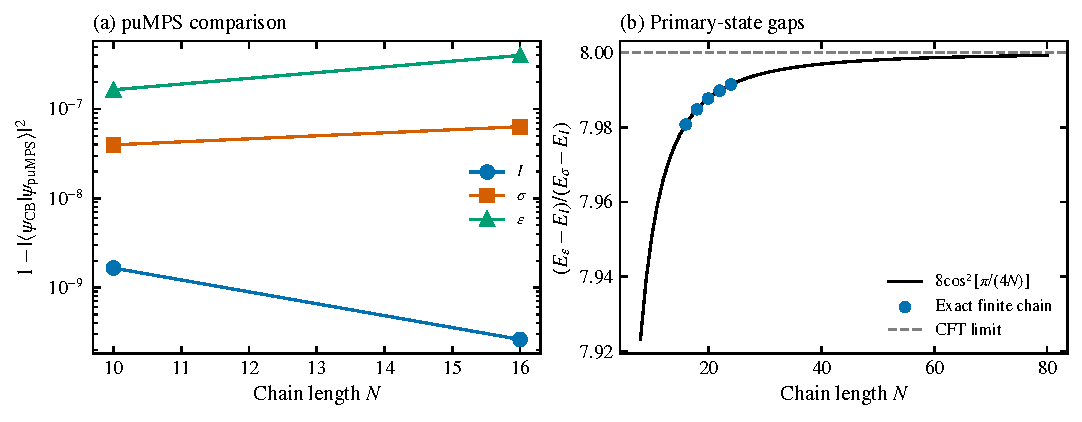
\includegraphics[width=\linewidth]{../figs/state_validation.pdf}
\caption{State validation at critical coupling and periodic spin boundaries.
(a) Squared-overlap infidelities against archived puMPS at
$(N,D_{\rm bond})=(10,8),(16,14)$, seeds $1244,1250$; $\sigma$ uses the
CB-seeded projection with solver tolerance $2\times10^{-12}$.
(b) Exact finite-chain gap ratios at $N=16,18,20,22,24$ and
Eq.~\eqref{eq:gaps}; the dashed line is the continuum value eight.
No interval length or mixture probability enters these whole-state tests.}
\label{fig:validation}
\end{figure}

\clearpage

\subsection{What was checked for the projected spin state}
\label{sec:ising-spin-validation}
For normalized vectors, define the energy error, eigenstate residual,
and squared overlap by
\begin{equation}
 \delta E=|\langle H\rangle-E_\sigma^{\rm exact}|,\qquad
 \eta=\|(H-\langle H\rangle)\ket{\sigma_N}\|_2,\qquad
 F=|\langle\sigma_{\rm ref}|\sigma_N\rangle|^2.
\end{equation}
The residual equals the square root of the energy variance. It tests
closeness to an eigenstate, but does not identify which eigenstate;
parity, translation and the exact lowest odd-sector energy supply that
identification. The interval comparison is
\begin{equation}
 e_\rho=\max_{1\leq\ell\leq\min(5,N/2)}
 \left\|\rho^{\rm Lanczos}_{\sigma,\ell}
       -\rho^{\rm covariance}_{\sigma,\ell}\right\|_F,
 \qquad \|B\|_F=\sqrt{\sum_{u,v}|B_{uv}|^2}.
\end{equation}
The following are the archived results in
\texttt{ising\_cb\_validation.csv}, rounded only for display.
That file evaluates the exact reference energy through the covariance;
using the equivalent trigonometric formula can change the last
roundoff digits of $\delta E$.
\begin{center}\small
\begin{tabular}{rrrrrr}\toprule
$N$ & $F_{\rm seed}$ & $\eta$ & $\delta E$ & $e_\rho$ & $|1-F|$\\\midrule
6 & .985928 & $1.54\,10^{-15}$ & $1.78\,10^{-15}$ & $1.82\,10^{-15}$ & $1.33\,10^{-15}$\\
8 & .982894 & $6.11\,10^{-15}$ & $5.33\,10^{-15}$ & $1.61\,10^{-15}$ & $2.22\,10^{-15}$\\
10 & .980864 & $2.22\,10^{-13}$ & $0$ & $2.76\,10^{-15}$ & $0$\\
12 & .979404 & $1.99\,10^{-11}$ & $2.49\,10^{-14}$ & $2.47\,10^{-13}$ & $1.78\,10^{-15}$\\
16 & .977431 & $2.70\,10^{-12}$ & $4.26\,10^{-14}$ & $4.02\,10^{-14}$ & ---\\\bottomrule
\end{tabular}
\end{center}
Here $F_{\rm seed}=|\langle\sigma_N|q_1\rangle|^2$ measures how much
of the target was already in the seed. For $N\leq12$, $F$ compares
against the lowest three eigenpairs from a separate full-spin-space
Hamiltonian action with a random starting vector. That reference also
uses \texttt{eigsh}; it is a different state construction, not an
independent eigensolver implementation. No full-space overlap was
recorded at $N=16$, hence the dash. Values of $F$ exceeding one by
roundoff are reported as $|1-F|$, not negative infidelities; zero entries
are floating-point results, not proofs of exact arithmetic equality.

The separate \texttt{ising\_construction\_checks.csv} run tests
$|\langle\sigma|\sigma\rangle-1|$,
$\|(P+1)\sigma\|_2$, $\|(\mathsf T-1)\sigma\|_2$, and
$\max_{a=I,\eps}|\langle a|\sigma\rangle|$ on the same five sizes.
Their maxima are $9.99\times10^{-16}$, $0$,
$7.20\times10^{-13}$, and $0$, respectively. Parity and mutual
orthogonality are enforced by disjoint basis sectors, so those zeros
alone do not establish state accuracy.

For context, the archived puMPS $\sigma$ residuals are
$2.65\times10^{-3}$ at $(N,D_{\rm bond})=(10,8)$ and
$3.10\times10^{-3}$ at $(16,14)$. Their squared overlaps with the
reference are $0.9999999603$ and $0.9999999366$.
These comparisons favor the exact reference for this integrable model
and these supplied checkpoints. They do not bound the accuracy of
puMPS after further optimization or at a larger bond dimension.

\subsection{Large-chain contraction and entropy checks}
\label{sec:large-sanity}
Validation tests each link in the calculation, rather than only checking
the final entropy. The 119 larger-interval records are in
\texttt{large\_interval\_checks.csv}; the earlier 345 smaller-interval
checks remain in \texttt{extension\_checks.csv}.
\begin{center}
\begin{minipage}{\linewidth}\small
\captionsetup{type=table}
\begin{tabular}{p{.58\linewidth}rr}\toprule
Check & Count & Largest difference\\\midrule
Boson ten-site matrix versus full wavefunction enumeration,
$N=20$, all three primaries &3&$3.22\times10^{-15}$\\
Boson 100 versus 130 working digits, $N=20,128$, $\ell=10$
&6&$<2\times10^{-14}$\\
Boson partial traces of ten-site matrices versus direct Pfaffians,
$N=20,128$, $\ell=4,5,6,7$ &24&$1.12\times10^{-16}$\\
Ising partial traces versus direct covariance reductions,
$N=32,82,128$, $\ell=4,5,6,7$ &36&$1.23\times10^{-15}$\\
Ising energies versus exact finite-chain formulas,
$N=32,82,128$ &9&$2.85\times10^{-14}$\\
Ising matrix entries between opposite parity sectors, $\ell=10$
&9&$0$\\
Symmetry-block versus full-matrix directed entropy, $\ell=10$
&2&$1.96\times10^{-14}$\\
Entropy threshold $10^{-15}$ versus $10^{-16}$, $\ell=10$
&30&$3.37\times10^{-13}$\\\bottomrule
\end{tabular}
\caption{Large-chain contraction and entropy checks. Counts give
the number of comparisons in each test family; sizes, interval lengths
and primary-state coverage are specified in the first column. Matrix
errors are maximum absolute entrywise differences; energy and entropy
errors are absolute scalar differences. The precision row reports a
validation-tolerance bound on the final double-precision matrices.}
\label{tab:large-validation}
\end{minipage}
\end{center}
Matrix differences in Table~\ref{tab:large-validation} mean the largest absolute entrywise
difference $\max_{u,v}|\rho^{(1)}_{uv}-\rho^{(2)}_{uv}|$; energy and
entropy differences are absolute scalar differences. Precision comparisons
refer to the final complex double-precision matrices, and the displayed
bound is their validation tolerance. The exact zeros refer to the
implemented parity-block structure, not a general error bound.

The full-matrix entropy checks use boson $ss\mid3s,s$ at $N=20$ and
Ising $\sigma\mid\eps$ at $N=82$. The threshold comparison covers all
six directions at $N=20,128$ for the boson and $N=32,82,128$ for Ising.
No mixture is replaced by a covariance-only approximation. The generation
stage independently checks trace, Hermiticity, and minimum eigenvalue for
all 294 state--interval combinations in the requested grid; these records
are in \texttt{large\_interval\_quality.csv}. The 180 observations shared
with the preceding grid retain their original stored values.

The exact contractions remove sampling and variational errors from the
present finite-lattice calculation. They do not remove the physical
dependence on $N$, $\ell$, or the fixed finite endpoint $W=10^8$.
The comparison with CFT in Sec.~\ref{sec:extension} keeps these physical
limitations distinct from numerical contraction accuracy.


Table~\ref{tab:large-validation} lists all eight families of the 119 checks, including
their sizes, norms, and errors. In particular, the $N=20$,
$\ell=10$ boson comparison tests every matrix element of all three
states against full wavefunction enumeration, with maximum error
$3.22\times10^{-15}$. This tests off-diagonal phases as well as
normalization. At $N=128$, where full enumeration is impractical,
increased working precision and agreement between direct and cached
contractions test numerical stability. They share the same algebraic
formula and therefore do not constitute an independent large-$N$
wavefunction proof. The algebra is derived in Sec.~\ref{sec:boson-contraction} and independently
tested at the sizes where enumeration is possible.

For Ising, finite-chain energies, covariance purity, zero-mode parity,
and agreement with smaller full vectors test distinct parts of the
construction. A partial trace of a ten-site matrix is also compared
with reconstruction from the directly restricted covariance. Entropy
checks then compare full-matrix and symmetry-block calculations, and
vary the eigenvalue threshold. Trace, Hermiticity and positivity are
necessary checks; agreement with an independently constructed state
is the stronger check. These tests certify the finite-lattice
calculation at the stated precision, not the absence of continuum
cutoff effects or unknown small-interval corrections.

\subsubsection{Endpoint checks for the extension through \texorpdfstring{$N=256$}{N=256}}
\label{sec:n256-sanity}
Before generating the new sizes, we tested all three states of each CFT
at $N=256$ and $\ell=10$. The 70 records in
\texttt{larger\_size\_checks.csv} test the same contraction in the new
size range. In addition to the matrix and entropy differences defined
in Table~\ref{tab:large-validation}, define
\begin{equation}
 e_G=\max_{r,s}|(G^2+\id)_{rs}|,\qquad
 e_P=|(-1)^N\operatorname{Pf}(G)-P|,\qquad
 e_+=\max(0,-\lambda_{\min}(\rho_A)).
 \label{eq:n256-diagnostics}
\end{equation}
Here $e_G$ tests purity of the full-chain Ising covariance, $e_P$ tests
its parity, and $e_+$ measures a negative eigenvalue caused by numerical
error. The remaining matrix-quality errors are $|\Tr\rho_A-1|$ and
$\max_{u,v}|(\rho_A-\rho_A^\dagger)_{uv}|$.
\begin{center}
\begin{minipage}{\linewidth}\small
\captionsetup{type=table}
\begin{tabular}{p{.61\linewidth}rr}\toprule
Check at $N=256$ & Count & Largest error\\\midrule
Ising exact finite-chain energies &3&$5.69\times10^{-14}$\\
Ising full covariance purity $e_G$ &3&$3.11\times10^{-15}$\\
Ising full-state parity $e_P$ &3&$5.96\times10^{-14}$\\
Ising partial traces versus direct covariance, $\ell=4,6$ &6&$5.42\times10^{-16}$\\
Boson 100 versus 130 digits, $\ell=10$ &3&$<2\times10^{-14}$\\
Boson partial traces versus direct Pfaffians, $\ell=4,6$ &6&$1.39\times10^{-16}$\\
Trace, Hermiticity and $e_+$, both CFTs, $\ell=10$ &18&$2.19\times10^{-16}$\\
Entropy cutoff $10^{-15}$ versus $10^{-16}$, $\ell=4,10$ &24&$7.93\times10^{-14}$\\
Symmetry-block versus full-matrix entropy, $\ell=4,10$ &4&$1.67\times10^{-14}$\\\bottomrule
\end{tabular}
\caption{All 70 endpoint checks for the extension to $N=256$. State
checks cover all three primaries per model; entropy-threshold checks
cover all six directions. Full-matrix comparisons use Ising
$\sigma\mid\eps$ and boson $ss\mid3s,s$. Errors use
Eq.~\eqref{eq:n256-diagnostics} and the entrywise/scalar conventions of
Table~\ref{tab:large-validation}. The precision row gives the validation
tolerance for final complex double-precision matrices, not a claim of
100-digit precision in the returned matrix.}
\label{tab:n256-validation}
\end{minipage}
\end{center}
All checks passed. The additional production run records trace,
Hermiticity and minimum eigenvalue for all $8\times3\times7\times2=336$
new state/interval combinations in \texttt{larger\_size\_quality.csv}.
It appends 672 directed relative entropies while preserving all 1200
earlier observations. The high-precision comparison shares the same
algebra and tests numerical stability; it is not an independent
full-wavefunction check at $N=256$.

\subsection{Reading route and attribution}
\begin{enumerate}
\item \textbf{Ising block states and the spin-primary limitation.}
Read Montes et al.~\cite{Montes2017}, Sec.~VIII, Eqs.~(55)--(62),
for the homogeneous even-sector block and its fermion ground state;
Appendix C, Eqs.~(133)--(137), supplies spin/fermion conventions.
Sec.~X, Eqs.~(73)--(75), constructs the energy-primary endpoint block.
The discussion after Eq.~(79) explains the difficulty with proposed
odd-sector endpoint states. Our summed-spin seed and odd-sector
projection, Eqs.~\eqref{eq:sigmaseed}--\eqref{eq:projection}, are a
project adaptation. They are not a published closed block formula for
$\sigma$.
\item \textbf{Lanczos projection.}
The algorithmic reference is the ARPACK guide~\cite{ARPACK}; the
direct implementation contract is \texttt{eigsh}~\cite{ScipyEigsh}.
The three-term recurrence and Rayleigh--Ritz selection are written out
in Appendix~\ref{sec:sigmamethod}. Our call uses \texttt{k=1},
\texttt{which="SA"}, \texttt{v0=seed}, and \texttt{tol=2e-12}.
It leaves \texttt{ncv} and \texttt{maxiter} at their defaults: for the
tested odd-sector dimension $d=2^{N-1}$, these are $20$ and $10d$.
No shift-invert transformation is requested. The API parameter
\texttt{sigma} denotes a spectral shift and is unrelated to our
primary-state name. The recorded environment uses SciPy 1.17.1;
the linked 1.17-series API describes these parameters.
\item \textbf{Large Ising chains.}
Read Peschel and Eisler~\cite{PeschelEisler}, Sec.~3.3(II),
Eqs.~(14)--(18), including the following Majorana paragraph.
It explains why a subsystem of a quadratic-fermion eigenstate is
determined by restricted correlations. Our explicit parity and zero-mode
selection precedes that reduction. Match the Majorana basis before
matching signs: we use
$\langle a_ra_s\rangle=\delta_{rs}-iG_{rs}$, whereas the review writes
$\delta_{rs}+i\Gamma_{rs}$ and chooses a different sign for one Majorana
per site. After aligning the basis, $G=-\Gamma$.
The Gaussian statement applies to each Ising primary; the mixture in
Eq.~\eqref{eq:large-target} is evaluated as a full matrix.
\item \textbf{Large compact-boson chains.}
Read St\'{e}phan and Pollmann~\cite{Stephan}, Appendix A.1,
Eqs.~(A5)--(A11), for the confluent Vandermonde determinant and
discrete Pfaffian normalization. Appendix A.2, Eqs.~(A14)--(A15),
introduces site weights for diagonal observables. Their site count $L$
and particle count $N$ are our $N$ and $M$. Their diagonal calculation
can discard amplitude phases. Our off-diagonal interval matrix cannot:
Eq.~\eqref{eq:pf-rdm} retains the bra and ket factors explicitly.
The finite-$W$ extension, bordered contraction, tridiagonal solve,
and reuse of repeated minors are developed in Sec.~\ref{sec:boson-contraction}, and are
checked against explicit vertex-state sums.
\item \textbf{Pfaffian signs and numerical evaluation.}
Wimmer~\cite{Wimmer}, Eqs.~(4) and (5), gives the first-row expansion
and congruence identity. These justify the cached recursion and block
elimination used here. Sec.~II A, Eqs.~(15)--(18), explains pivoted
antisymmetric elimination, the basis of our scalar Pfaffian helpers.
Our code implements those elementary updates using NumPy or mpmath;
it does not call the paper's software package. Caching the minors and
sharing multiplicity factors are implementation choices in this project.
\end{enumerate}

\subsection{From a formula to its source function}
All Python paths in this table are relative to
\texttt{src/conformal\_blocks/}; the method functions have source
references in their docstrings. A reduced density matrix is abbreviated
RDM in function and data-file names.
\begin{center}\small
\begin{tabular}{>{\raggedright\arraybackslash}p{.35\linewidth}>{\raggedright\arraybackslash}p{.57\linewidth}}\toprule
Operation & File and functions\\\midrule
Block vacuum and projected $\sigma$
&\path{ising.py}: \path{fusion_blocks}, \path{sigma_from_cb},
\path{hamiltonian_action}, \path{energy_diagnostics}\\
Quadratic sectors, zero modes and Eq.~\eqref{eq:large-ising-rdm}
&\path{ising.py}: \path{majorana_covariance}, \path{pfaffian},
\path{gaussian_rdm}; direct comparison: \path{dense_rdm}\\
Explicit compact-boson amplitudes
&\path{boson.py}: \path{vertex_state}, \path{sector_rdm}\\
Eqs.~\eqref{eq:pf-small} and \eqref{eq:pf-rdm}
&\path{boson_pfaffian.py}: \path{jastrow_rdm},
\path{_tridiagonal_solve}, \path{pfaffian_mp}, \path{_cached_density}\\
Shorter intervals and exact mixture entropy
&\path{boson_pfaffian.py}: \path{block_rdms};
\path{symmetry_entropy.py}: \path{sectors}, \path{directed_entropies}\\
Validation and current-grid generation
&\path{method_sanity.py}, \path{extension_checks.py},
\path{large_interval_checks.py}, \path{large_intervals.py}\\\bottomrule
\end{tabular}
\end{center}

\subsection{A short reproduction run}
From the root of the full reproducibility project, using a Python
environment containing NumPy, SciPy and mpmath, run
\begin{verbatim}
export PYTHONPATH=src
export OPENBLAS_NUM_THREADS=1
python -m conformal_blocks.method_sanity \
  --output method_sanity.json
\end{verbatim}
This script constructs $\sigma$ at $N=12$, checks its energy, residual,
symmetries and four-site reduction, and tests all three primaries at
$N=12,128$ for both CFTs with $\ell=4$. The boson checks compare the
cached 100-digit calculation with direct 130-digit Pfaffians, and at
$N=12$ with explicit vertex amplitudes. It also compares both entropy
implementations. Every check writes its error, tolerance, parameters
and pass flag. The executed result is archived as
\texttt{data/method\_sanity.json}; all 55 checks passed. This compact
reproduction supplements the archived 345 earlier checks and 119
ten-site checks, without replacing them or rerunning any fits.
